\section{问题二：变物性双向耦合的全过程烘干模型}

\subsection{相对问题一的改动}

本问保留公共模型一章的控制方程、边界条件与初始条件，也保留问题一的固定求解域 $R=2$~cm，
只把物性关系由式~\eqref{eq:prop_app2} 换成式~\eqref{eq:prop_app3}。这一处改动使
式~\eqref{eq:energy} 与式~\eqref{eq:moisture} 由弱联系变为双向耦合：$\rho$、$c_p$、$k$
随含水率变化，扩散系数同时随含水率与温度变化。改动虽只在系数，数学类型却由
「线性温度场 + 非线性水分场」变成「两个互相牵动的非线性方程」，求解上必须使用
公共模型一章所述的算子分裂与迭代复核，不能沿用问题一的先算温度再算水分的做法。

耦合还改变了物性本身的量程。将式~\eqref{eq:prop_app3} 代入本问实际出现的含水率区间，
密度、比热容与导热系数都随失水而下降，同时扩散系数受两个方向的相反影响：
含水率下降使其减小、温度上升使其增大。哪一方占优决定干燥的快慢，
这一点在结果讨论中用实际计算的物性联动来回答。

时间步长取 $\Delta t=1$~s，报表窗口为题目要求的 $0$--$3$~h。需要强调的是 $3$~h
只是报表要求，并非过程终止：同一次求解一直推进到含水率达标为止，
其终止时刻由下一章的判据给出。

\subsection{前 3 小时的温度与含水率分布}

按题目要求的时刻与位置整理，见表~\ref{tab:p2_T} 与表~\ref{tab:p2_C}。

\begin{table}[H]
\centering
\caption{全过程模型下药材内部温度（$^\circ$C）}\label{tab:p2_T}
\begin{tabular}{cccccc}
\toprule
时间 (h) $\backslash$ 距中心距离 (cm) & 0 & 0.5 & 1 & 1.5 & 2 \\
\midrule
0.5 & 32.1908 & 32.3836 & 32.9673 & 33.9620 & 35.4141 \\
1.0 & 40.3817 & 40.5536 & 41.0606 & 41.8785 & 42.9980 \\
1.5 & 45.8462 & 45.9343 & 46.1925 & 46.6047 & 47.1398 \\
2.0 & 48.4498 & 48.4876 & 48.5980 & 48.7732 & 49.0031 \\
2.5 & 49.4667 & 49.4789 & 49.5134 & 49.5653 & 49.6609 \\
3.0 & 49.8495 & 49.8553 & 49.8745 & 49.9101 & 49.9664 \\
\bottomrule
\end{tabular}
\end{table}

\begin{table}[H]
\centering
\caption{全过程模型下药材内部水分浓度（kg/kg）}\label{tab:p2_C}
\begin{tabular}{cccccc}
\toprule
时间 (h) $\backslash$ 距中心距离 (cm) & 0 & 0.5 & 1 & 1.5 & 2 \\
\midrule
0.5 & 2.5499 & 2.5488 & 2.5254 & 2.3260 & 1.6486 \\
1.0 & 2.5255 & 2.4946 & 2.3578 & 2.0231 & 1.4710 \\
1.5 & 2.3859 & 2.3255 & 2.1344 & 1.8020 & 1.3475 \\
2.0 & 2.1708 & 2.1084 & 1.9236 & 1.6259 & 1.2310 \\
2.5 & 1.9566 & 1.9006 & 1.7360 & 1.4720 & 1.1166 \\
3.0 & 1.7662 & 1.7166 & 1.5702 & 1.3332 & 1.0080 \\
\bottomrule
\end{tabular}
\end{table}

温度方面，中心由 $0.5$~h 的 $32.1908~^\circ$C 升至 $3$~h 的 $49.8495~^\circ$C，
已逼近烘房平台温度 $50.165~^\circ$C；同一时刻中心与表面之差由 $3.22~^\circ$C
收窄到 $0.12~^\circ$C。也就是说药材在约 $3$~h 后基本进入等温状态，此后温度不再是限制因素。
含水率方面，$3$~h 时中心仍有 $1.7662$~kg/kg，距 $0.15$~kg/kg 的目标相去甚远，
而表面已降至 $1.0080$~kg/kg。两者对比给出一个重要判断：干燥的限制环节不是供热，
而是水分从芯部迁移到表面的内部阻力。这也解释了题目所述烘干需持续两三天的量级。

与问题一相比，中心含水率在 $3$~h 内下降了 $0.78$~kg/kg，而问题一在 $0.5$~h 内
几乎未动。图~\ref{fig:q2_profiles} 给出本问剖面的演化形态。

\begin{figure}[H]
  \centering
  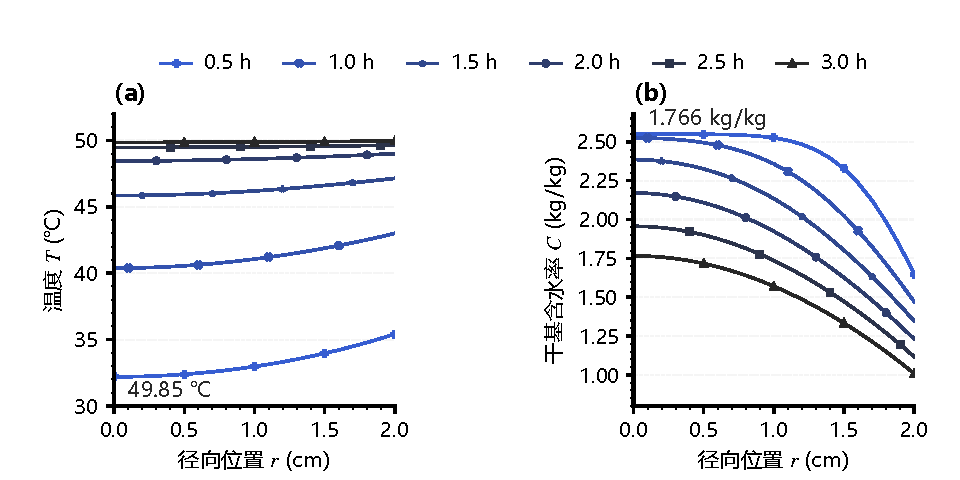
\includegraphics[width=0.9\textwidth,height=0.8\textheight,keepaspectratio]{../figures/fig_q2_profiles.pdf}
  \caption{问题二温度与含水率的径向剖面}
  \label{fig:q2_profiles}
\end{figure}

温度剖面在 $1.5$~h 之后已趋于平坦，各位置之差不足 $1~^\circ$C；含水率剖面则持续下移并
逐渐由「仅表层弯折」变为「整体倾斜」，说明水分下降已推进到可观深度而非局限于表层。
两个面板的时间尺度差异再次印证前段的判断：温度场先达到准稳态，水分场在此之后才是主角。

把两个场在整个时间窗上铺开，可与问题一作同一标尺的对照，见图~\ref{fig:q2_spacetime}。

\begin{figure}[H]
  \centering
  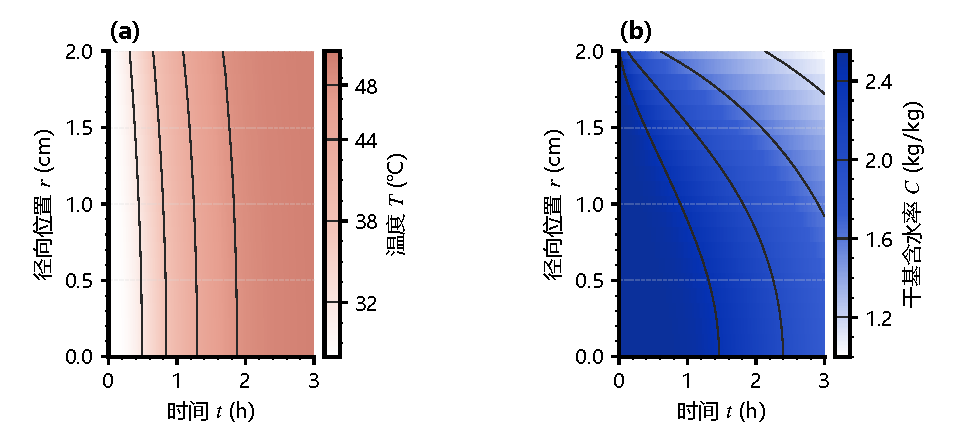
\includegraphics[width=0.9\textwidth,height=0.8\textheight,keepaspectratio]{../figures/fig_q2_spacetime.pdf}
  \caption{问题二温度场与含水率场的时空分布}
  \label{fig:q2_spacetime}
\end{figure}

温度场在约 $1$~h 内基本追平空气平台温度，其后色阶不再变化；含水率场呈现一条由表面
向中心推进的干燥前沿，前沿位置随时间内移。与图~\ref{fig:q1_spacetime} 相比，
含水率的可见变化区已由「表层窄带」扩展到「全域」，量级的改变来自物性关系的更换而非
时间窗的延长。这一点需要在同一时刻上比较才能确认，见图~\ref{fig:q12_contrast}。

\begin{figure}[H]
  \centering
  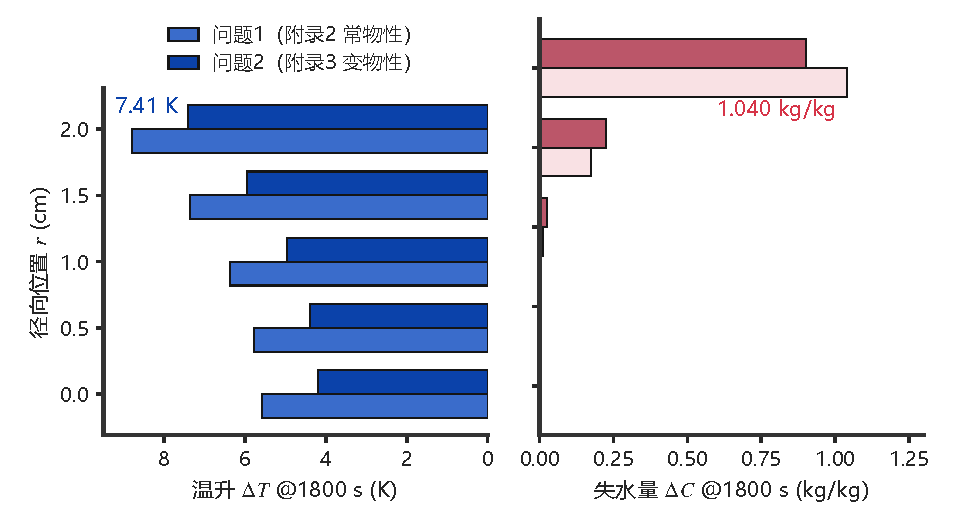
\includegraphics[width=0.9\textwidth,height=0.8\textheight,keepaspectratio]{../figures/fig_q12_contrast.pdf}
  \caption{问题一与问题二在 $t=1800$~s 的增量对比}
  \label{fig:q12_contrast}
\end{figure}

图中取同一时刻 $t=1800$~s 背靠背比较两问的温升与含水率降幅。温升的差异始终在数摄氏度量级，
而含水率降幅在中心处相差近一个量级（$1.0\times10^{-5}$ 对 $7.9\times10^{-5}$~kg/kg）；
表面处则出现符号反转：问题一的表面降幅 $1.039$~kg/kg 反而大于问题二的
$0.901$~kg/kg。这一「内部放大、表面反转」的格局说明物性关系的更换主要改写了水分方程的
内部输运能力，而不是表面的传质条件——表面通量由 $h_m$ 与表面浓度差决定，两问的 $h_m$ 相同，
问题二表面失水略少恰恰因为内部补水更快、表面浓度维持得更高。

\subsection{耦合关系的实际表现}

前文的判断需要落到物性本身。图~\ref{fig:q2_properties} 把全程节点场按含水率分箱，
给出四项物性的联动。

\begin{figure}[H]
  \centering
  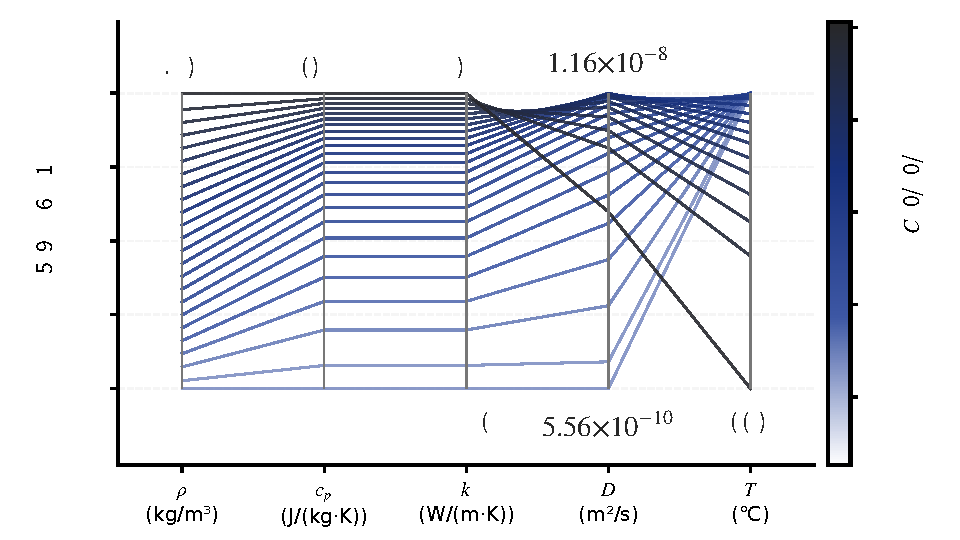
\includegraphics[width=0.9\textwidth,height=0.8\textheight,keepaspectratio]{../figures/fig_q2_properties.pdf}
  \caption{附录 3 四项物性随含水率的联动}
  \label{fig:q2_properties}
\end{figure}

随含水率由 $2.53$ 降到 $0.13$~kg/kg，密度由 $973.7$ 降到 $666.8$~kg/m$^3$、
比热容由 $3411$ 降到 $1765$~J/(kg$\cdot$K)、导热系数由 $0.482$ 降到
$0.254$~W/(m$\cdot$K)，三者同向下降。扩散系数的最低值 $5.70\times10^{-10}$~m$^2$/s
出现在最低含水率箱，说明在含水率与温度的两个相反影响中，含水率的影响占优：
即使后期温度已升至平台值，扩散系数仍随失水而下降。这正是干燥后期速率持续减慢、
达标时间被显著拉长的机制来源。热风干燥试验中由失水曲线反演有效扩散系数与活化能，
所得量级与本文所用经验式一致\upcite{Doymaz2011}。

耦合的另一侧面是求解轨迹在状态平面上的分布，见图~\ref{fig:q2_coupling_scatter}。

\begin{figure}[H]
  \centering
  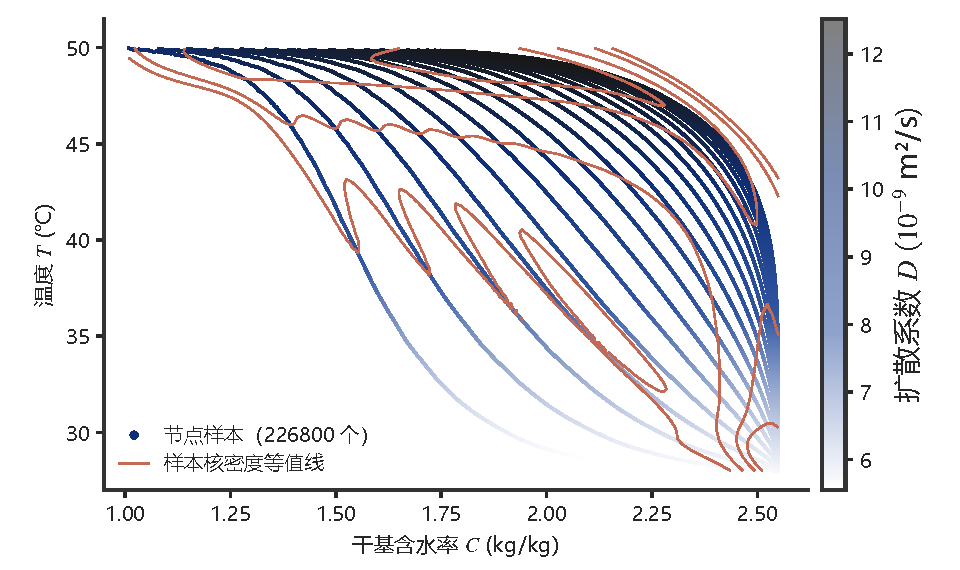
\includegraphics[width=0.9\textwidth,height=0.8\textheight,keepaspectratio]{../figures/fig_q2_coupling_scatter.pdf}
  \caption{问题二时空节点在含水率-温度平面上的分布}
  \label{fig:q2_coupling_scatter}
\end{figure}

$14801$ 个节点样本聚成两条带：升温初期的高含水率带，以及准平台温度下的降湿带。
两带交界处正是扩散系数变化最剧烈的区域，也是算子分裂次序最敏感的阶段。若此处用旧层温度
计算扩散系数，误差会直接进入后续全部时程。实际计算中 Picard 迭代最多 $3$ 次即收敛，
质量收支相对残差 $1.55\times10^{-14}$，说明该阶段的耦合已被正确处理。

按题目要求，全过程每隔 $1$~s、距中心每隔 $0.1$~cm 的温度与含水率完整结果保存于结果文件，
共 $204143$ 个时间行，覆盖从初始时刻到含水率达标的整个过程。
